\chapter{Stand van zaken}
\label{ch:stand-van-zaken}

% Tip: Begin elk hoofdstuk met een paragraaf inleiding die beschrijft hoe
% dit hoofdstuk past binnen het geheel van de bachelorproef. Geef in het
% bijzonder aan wat de link is met het vorige en volgende hoofdstuk.

% Pas na deze inleidende paragraaf komt de eerste sectiehoofding.

\section{JavaScript}
In deze sectie zal JavaScript besproken worden. Hier zal dieper ingegaan worden op zowel de historiek als op de eigenschappen van de populaire scripttaal.

\subsection{Historiek}
JavaScript werd in 1995 ontwikkeld door Brendan Eich, toen deze werkte bij het softwarebedijf Netscape Communications. Netscape Communications werd bekend door het ontwikkelen van de Netscape Navigator browser. Deze browser was in de jaren '90 de populairste browser en bleef op de markt tot 1 februari 2008. De taak van Eich was om een scripttaal te ontwikkelen voor deze web browser. 

Brendan Eich liet zich bij de ontwikkeling van JavaScript inspireren door drie andere scripttalen: Java, Scheme en Self. Aanvankelijk kwam JavaScript in maart 1995 op de markt onder een andere naam: Mocha. Enkele maanden later veranderde de scripttaal al van naam, het werd nu LiveScript. In december 1995 volgde er een licentieovereenkomst tussen Sun en Netscape Communications waardoor de naam weer aangepast werd, nu naar JavaScript.
Netscape Communications heeft JavaScript laten normeren door de European Computer Manufacturers Association(ECMA) om zo de taal als officiële norm erkend te krijgen. 
Deze gestandaardiseerde versie staat bekend als ECMAScript.

\subsection{Eigenschappen}
JavaScript is één van de populairste scripttalen in de afgelopen twintig jaar.
Bovendien is het ook één van de drie belangrijkste talen (zie figuur \ref{fig:Triade}) voor webdevelopers:
\begin{itemize}
\item HTML: inhoud van webpagina's
\item CSS: layout en stijl van webpagina's
\item JavaScript: maakt webpagina's interactief en zorgt voor een meer gebruiksvriendelijke ervaring.

\end{itemize}
\graphicspath{{./img/}}

\begin{figure}[H]
	\centering
	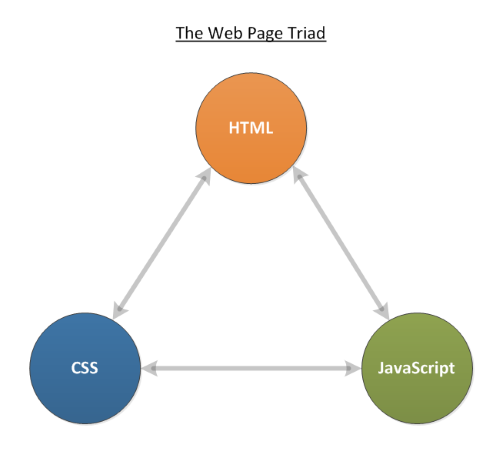
\includegraphics[width=0.6\linewidth]{triadJavaScript}
	\caption{Triade van de webpagina \autocite{itegrators2017}}
	\label{fig:Triade}
\end{figure}

Dankzij JavaScript is het mogelijk om de meeste elementen op een webpagina programmeerbaar te maken. Het wordt momenteel gebruikt op 95 procent van alle websites \autocite{W3Techs2019}. Het is ook de basis van andere scripttalen zoals TypeScript, waarvan Angular gebruik maakt.

Javascript wordt vaak verward met Java, maar dit is niet terecht. Ondanks dat beide talen enkele gelijkenissen vertonen, zijn er toch heel wat verschillen. De syntaxis van beide talen is gebaseerd op die van programmeertaal C. Samen met de naam van beide talen is dit de grootste gelijkenis. 

De verschillen zijn talrijk.
 Vooraleerst is Java een gecompileerde programmeertaal, terwijl JavaScript een geïnterpreteerde scripttaal is. Het verschil zit hem in de implementatie.  JavaScript kan direct geïnterpreteerd worden door de browser terwijl Java wordt gecompileerd naar bytecode aan de hand van een virtuele machine, namelijk de Java Virtual Machine (JVM). 

 Ten tweede is JavaScript loosely typed, dit wil zeggen dat we op voorhand niet moeten aangeven welke soort van informatie (boolean, string, int...) zal opgeslaan worden in een variabele. Dit zal pas gecontroleerd worden tijdens runtime. Java is strongly typed, hier moet het type steeds op voorhand gedeclareerd worden omdat de check reeds zal gebeuren bij compiletime. Dit maakt van JavaScript een meer flexibele taal maar helaas is JavaScript hierdoor ook gevoeliger voor bugs omdat de check pas later in het proces gebeurt.
 
 Een derde belangrijk verschil is dat van de concurrency. Java maakt gebruik van meerdere threads zodat het taken in parallel kan uitvoeren. JavaScript maakt gebruik van één main thread wat ervoor zorgt dat het in het algemeen trager werkt dan Java.
 
 Het laatste verschil is dat Java klasse gebaseerd is terwijl JavaScript prototype gebaseerd is. Bij klasse gebaseerde talen is er een top down hiërarchische structuur. 
 Een property  wordt gedefiniëerd in een klasse en zal overgeërfd worden door elke instantie van die klasse. Bij JavaScript is overerving prototypal, dit wil zeggen dat elk object kan erven van andere objecten.   
 
 \section{TypeScript}
 TypeScript is een open-source programmeertaal ontwikkeld door Microsoft. Het is een superset van JavaScript die ervoor zorgt dat statisch typen mogelijk wordt. Het werd in 2012 op de markt gebracht met de bedoeling om de ontwikkeling van grote applicaties eenvoudiger te maken. TypeScript wordt gecompileerd naar JavaScript wat ervoor zorgt dat gewone JavaScript applicaties ook geldige TypeScript applicaties zijn. 
 
 De voordelen van TypeScript ten opzichte van JavaScript zijn talrijk: het is een object-georiënteerde taal, compilation errors worden sneller gevonden door de TypeScript transpiler, het is een strongly-typed taal,... Bovendiendien is de populariteit van typescript enorm snel aan het stijgen. 
 
 De huidige versie van Typescript is TypeScript 3.4 en werd in maart 2019 uitgebracht.

\section{Framework}

Een software framework is een samenstelling van softwarecomponenten dat kan gebruikt worden bij het programmeren van applicaties. Het zal de tijd en kost voor het ontwikkelen van een applicatie aanzienlijk doen dalen. 
Het is een herbruikbaar raamwerk dat kan uitgebreid worden met zelf geschreven code. Software frameworks bestaan uit verschillende ondersteunende programma's, compilers, bibliotheken, tool sets en application programming interfaces (API).

Frameworks onderscheiden zich van gewone libraries aan de hand van drie kenmerken:

\begin{itemize}
	\item Inversion of control: Wanneer een methode uit een library wordt aangeroepen heeft de gebruiker de controle. Bij een framework is het het framework zelf dat de flow control bepaalt. 
	\item Uitbreidbaarheid: De gebruiker kan een framework uitbreiden of er gespecialiseerde code aan toevoegen om zo een specifieke functionaliteit toe te voegen. 
	\item Niet aanpasbare framework code: Hoewel de gebruiker het framework kan uitbreiden, mag hij de code niet aanpassen. Een framework volgt dus het open/closed-principe. 
	
\end{itemize}


\section{Component-gebaseerd Framework}
Een component-gebaseerd framework is een framework voor webapplicaties dat de verwerkingslogica opsplitst in verschillende onderdelen, genaamd componenten. 
Een component is dus een bouwsteen waaruit de applicatie is opgebouwd. Een component-gebaseerd framework bestaat uit veel verschillende componenten die variëren van heel klein tot heel groot zoals buttons, lijsten of volledige views. De component zorgt voor een eenvoudige configuratie van deze onderdelen. 


\section{Single Page Application}
Een Single Page Application (SPA) is een webapplicatie die draait op één enkele HTML webpagina. De HTML, CSS en JavaScript code wordt opgehaald in één laadactie van de pagina. De pagina zal daarna dynamisch bijgewerkt worden wanneer de gebruiker interageert met de webapplicatie (zie figuur \ref{fig:SPA}). Dankzij deze manier van werken is een Single Page Application vaak veel sneller dan een statische website, aangezien de statische website steeds opnieuw de inhoud moet laden. Alle JavaScript frameworks passen automatisch het Single Page Application concept toe. 

\begin{figure}[H]
	\centering
	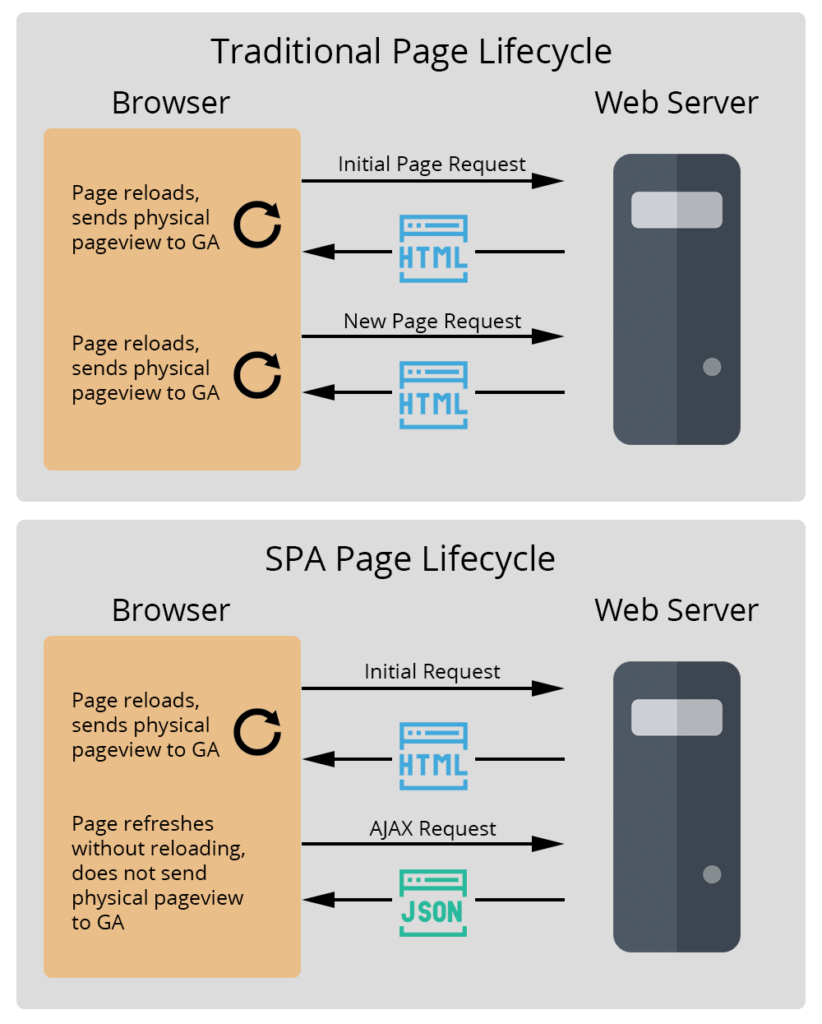
\includegraphics[width=0.5\linewidth]{spa-architecture}
	\caption{Statische website versus Single Page Application \autocite{E-nor2018}}
	\label{fig:SPA}
\end{figure}

\section{MVC}
De applicaties die opgebouwd zullen worden om beide frameworks te vergelijken zullen gebruik maken van het MVC(Model-View-Controller) patroon (zie figuur \ref{fig:Mvc} ). Daarom is het noodzakelijk om dit patroon kort te beschrijven.


Model View Controller is een ontwerppatroon dat een applicatie verdeelt in drie eenheden met verschillende verantwoordelijkheden:

	\textbf{Model}  \hspace{1cm} Het datamodel specifieert de logische structuur van de data in de applicatie. Het zal beschrijven hoe de data weergegeven wordt op niveau van de databank. Het datamodel beschrijft welke entiteiten verbonden zijn aan welke tabellen en hoe het zit met de relaties tussen deze datastructuren.   					\\ \\
	\textbf{View} \hspace{1cm} De view bepaalt hoe de data zal weergegeven worden op het scherm. Het doet geen verwerking van de gegevens maar wordt enkel gebruikt voor de interactie met de user. De userinterface-elementen worden allemaal gedefinieerd in dit onderdeel. 						\\	\\
	\textbf{Controller} \hspace{1cm} De controller verzorgt de interactie tussen de view en het model. De controller bestaat uit actions die reageren op de handelingen van de gebruiker. Aan de hand van die actions wordt het juiste model gebruikt en de passende view weergegeven.  			\\	\\
De voordelen van dit patroon zijn talrijk: de applicatie zal makkelijker uitbreidbaar worden, het ontwikkelingsproces zal sneller verlopen, dubbele code wordt vermeden, een model kan verschillende views toegewezen krijgen en modificatie van één van de drie eenheden zal geen invloed hebben op de andere eenheden.

\begin{figure}[H]
	\centering
	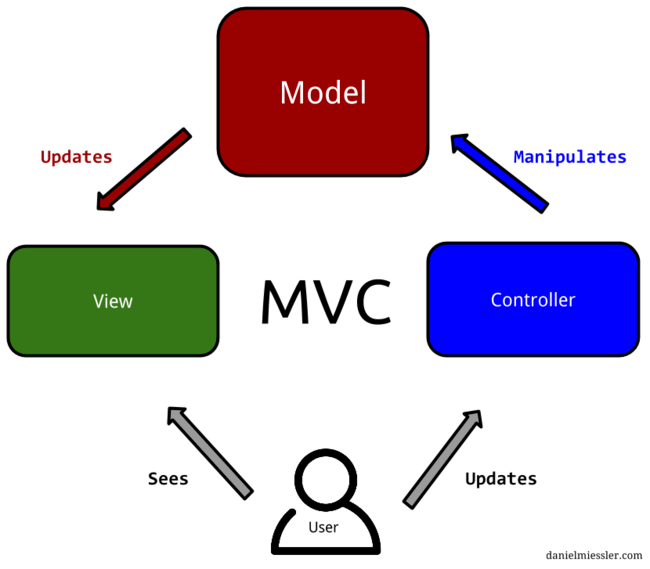
\includegraphics[width=0.6\linewidth]{MVC}
	\caption{Overzicht van het MVC patroon \autocite{DanielMissler2017}}
	\label{fig:Mvc}
\end{figure}

\section{Angular}
"Angular is a platform that makes it easy to build applications with the web. Angular combines declarative templates, dependency injection, end to end tooling, and integrated best practices to solve development challenges. Angular empowers developers to build applications that live on the web, mobile, or the desktop." \autocite{Angular2019} 

Angular is een front-end framework gebaseerd op TypeScript dat onderhouden wordt door het Angular Team van Google. Het is een volledig herschreven versie van AngularJS.
De belangrijkste bouwstenen van een Angular applicatie zijn de modules, componenten en services (zie figuur \ref{fig:Angular-Module-Component}).


\begin{figure}
\begin{lstlisting}[]
// imports
import { BrowserModule } from '@angular/platform-browser';
import { NgModule } from '@angular/core';
import { FormsModule } from '@angular/forms';
import { HttpClientModule } from '@angular/common/http';

import { AppComponent } from './app.component';
import { ItemDirective } from './item.directive';


// @NgModule decorator with its metadata
@NgModule({
declarations: [
AppComponent,
ItemDirective
],
imports: [
BrowserModule,
FormsModule,
HttpClientModule
],
providers: [],
bootstrap: [AppComponent]
})
export class AppModule { }
\end{lstlisting}
\caption{Angular root module voorbeeld}
\end{figure}


\subsection{Module}
Angular is een modulair framework, het is dus opgebouwd uit modules. Een module in Angular refereert naar een plaats waar componenten, directives, pipes en services gegroepeerd kunnen worden (zie figuur \ref{fig:Angular-Module-Component}). 
Het modulariteitssysteem van Angular heet NgModules en kan zowel functionaliteiten importeren die door andere NgModules worden geëxporteerd als zelf functionaliteiten exporteren. 
\\ \\
Elke Angular app heeft minstens één NgModule klasse, genaamd de root module. Gewoonlijk wordt deze de AppModule genoemd en wordt deze geplaatst in een file met de naam app.module.ts. Deze module zorgt voor het opstarten van de applicatie. 

\begin{figure}[H]
	\centering
	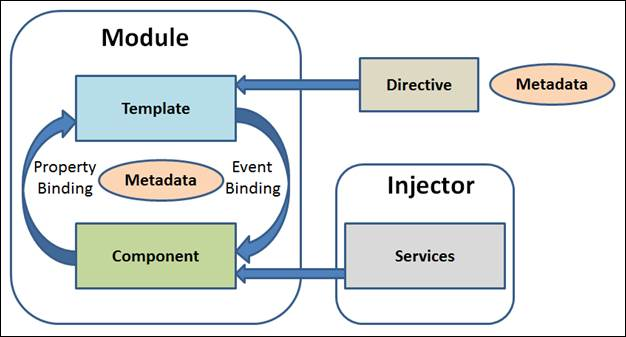
\includegraphics[width=0.6\linewidth]{Angular-Module-Component}
	\caption{Overzicht van de Angular bouwstenen \autocite{Trivedi2016}}
	\label{fig:Angular-Module-Component}
\end{figure}

\textbf{NgModule metadata} \hspace{1cm} Een NgModule wordt steeds gedefinieerd door een klasse met de decorator @NgModule(). Deze decorator is een functie dat een metadata object gebruikt om de module te beschrijven. De belangrijkste attributen van dit object zijn de volgende: 
\begin{itemize}
	\item declarations: De componenten, directives en pipes die toebehoren aan deze module.  
	\item exports: De subset van declaraties dat andere NgModules moeten kunnen importeren. 
	\item imports: Andere modules die nodig zijn binnen deze NgModule. 
	\item providers: Services die deze NgModule gebruikt. Providers die op dit niveau worden gedeclareerd kunnen over de hele app gebruikt worden. Het is echter ook mogelijk om providers te declareren op niveau van componenten, wat vaak een betere optie is.
	\item bootstrap: Dit attribuut moet enkel ingesteld worden door de root NgModule. Het bepaalt de algemene view die alle andere views beheert.
\end{itemize}

Het NgModule systeem is verschillend van het JavaScript module systeem voor het beheren van collecties van JavaScript objecten. Het NgModule systeem en het JavaScript module systeem zijn complementaire systemen die kunnen gecombineerd worden bij het schrijven van applicaties. 

\subsection{Component}
Componenten zijn de eenvoudigste bouwstenen van een angular applicatie. Ze beheren een deel van het scherm dat bekend staat als een view. Binnen een MVC context zouden ze omschreven worden als een controller. Een component behoort steeds toe aan een NgModule, zodanig dat het beschikbaar kan zijn voor een andere component of applicatie. 

Een component heeft verschillende lifecycle hooks (zie figuur \ref{fig:lifecyclehooks}), zoals de ngOnInit(). In elk van deze lifecycle hooks kan je applicatie bepaalde acties uitvoeren. Angular zal componenten automatisch aanmaken, updaten en verwijderen terwijl de gebruiker navigeert door de applicatie. 

\begin{figure}[H]
	\centering
	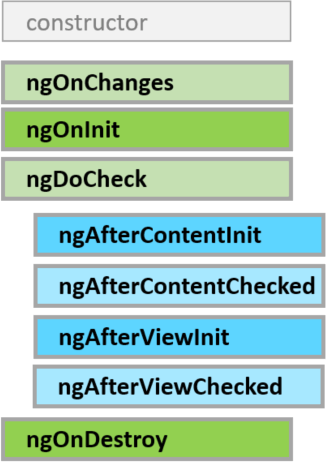
\includegraphics[width=0.6\linewidth]{lifecyclehooks}
	\caption{De lifecycle hooks \autocite{dartlang2019}}
	\label{fig:lifecyclehooks}
\end{figure}

\textbf{Component metadata} \hspace{1cm} Een component klasse is een klasse die wordt geïdentificeerd aan de hand van de @Component decorator. Deze klasse zal de metadata van de component bevatten. De metadata van een component laat aan Angular weten waar ze de bouwstenen kan vinden die nodig zijn om de component en zijn view aan te maken. De combinatie van een component met zijn template zorgen voor een view. 
De belangrijkste configuratieopties van een component zijn de volgende:
\begin{itemize}
	\item selector: De selector vertelt Angular om een component te maken op de plaats waar het de corresponderende tag vindt in de HTML. 
	\item templateUrl: Het adres van de HTML template die gelinkt is aan de component. Dit adres is relatief aan de module. 
	\item providers: Services die door deze component gebruikt worden. Deze worden weergegeven in een array. 
\end{itemize}

\textbf{Template en views} \hspace{1cm} De view van een component wordt steeds gedefiniëerd aan de hand van een bijhorende template. De template is een HTML form dat Angular de informatie doorgeeft die nodig is om de component weer te geven. Views worden hiërarchisch geordend, waardoor het mogelijk is om volledige onderdelen van de user interface aan te passen of te verbergen. De template die rechtstreeks geassocieerd is met de component noemt men de host view. Deze host view kan embedded views bevatten die beheerd worden door andere componenten. Deze componenten kunnen zich in een andere NgModule bevinden. 

\textbf{Data binding} \hspace{1cm} Databinding is het proces dat zorgt voor een connectie tussen de interface van de applicatie en het model. Wanneer de data verandert van waarde, zal de interface ook aangepast worden. Het opstellen van zo een mechanisme is een moeilijke en arbeidsintensieve taak. Gelukkig is dit met Angular eenvoudig te implementeren. Angular voorziet zelfs in two-way binding, wat inhoudt dat ook het model kan aangepast worden via de interface, bijvoorbeeld door het invullen van een formulier. Angular voorziet in drie verschillende manieren om data te binden:
\begin{itemize}
	\item interpolation: Techniek om waardes te binden aan een User Interface element.
	Deze techniek kan enkel gebruikt worden bij one-way binding van component naar view. Interpolation gebruikt als scheidingsteken de dubbele accolades \{\{ en \}\}. Interpolation is een speciale syntax die door Angular wordt geconverteerd naar property binding.
	\item property binding: Techniek om waardes te binden aan DOM attributen van de HTML elementen. Zo kunnen de attributen van view elementen ingesteld worden, zoals de bron van een afbeelding. Net zoals interpolation kan deze techniek enkel gebruikt worden bij one-way binding van component naar view. De scheidingstekens van property binding zijn de vierkante haakjes [ en ].
	\item event binding: Wanneer users interageren met de applicatie zoals een click of een actie van het toetsenbord kan dit via event binding opgevangen worden. Event binding is een one-way binding maar in tegenstelling tot de voorgaande technieken werkt deze van view naar component. De scheidingstekens van event binding zijn de ronde haakjes ( en ). 
\end{itemize}
Door bovenstaande one-way binding technieken te combineren is het in Angular mogelijk om two-way binding te bekomen. 

\textbf{pipes} \hspace{1cm} Dankzij pipes is het mogelijk om waardes die worden weergegeven in de template HTML te transformeren. Een klasse met de @Pipe decorator definieert een functie die input waardes transformeert naar output waardes voor een view. Angular voorziet al enkele pipes zoals de date pipe of de currency pipe, maar het is ook mogelijk om zelf pipes te maken. Om een transformatie in een HTML template te specifiëren gebruikt men de pipe operator: |. 

\textbf{directives} \hspace{1cm} De templates van Angular zijn dynamisch. Wanneer ze weergegeven worden zullen ze getransformeerd worden volgens de instructies die meegegeven worden door directives. Een directive is een klasse met de @Directive() decorator. Er zijn twee soorten directives: structural en attribute. 

De structural directives kunnen elementen verwijderen, toevoegen of vervangen in de DOM. Er zijn twee automatisch ingebouwde structural directives: de NgFor die iteraties uitvoert en de nfIf die een check uitvoert op condities.

De attribute directives kunnen het gedrag of het voorkomen van een bestaand element aanpassen. In de templates lijken ze op gewone HTML attributen, vandaar ook de naam. 
Een voorbeeld van een attribute directive is de ngModel die zorgt voor two-way data binding. Het verandert het gedrag van een bestaand element zoals bijvoorbeeld <input>. 

\subsection{Service}
Service is een brede naam voor elke waarde, functie of feature dat een applicatie nodig heeft. Een service is een klasse met een zeer specifiek doel. Het grote verschil tussen een component en een service is het feit dat een component gelinkt is aan een view, terwijl een service dat niet is. \\
Een component kan bepaalde taken delegeren aan een service, zoals het ophalen van data van een server of het valideren van de input van een gebruiker. De services kunnen hergebruikt worden over de hele applicatie waardoor er minder redundante code zal ontstaan. Bovendien zorgen ze er ook voor dat componenten niet te groot worden. 

\textbf{dependency injection} \hspace{1cm} services worden geïnjecteerd in een component, waardoor deze components toegang hebben tot die service klasse.De service klasse heeft geen specifieke decorator, maar maakt gebruik van de @Injectable() decorator. Deze zorgt ervoor dat Angular de klasse kan injecteren in een component als een dependency. Een dependency hoeft geen service te zijn, maar kan evenwel een functie of een waarde zijn. 

Wanneer Angular ontdekt dat een component een dependency heeft op een service, zal het eerst nakijken of er al bestaande instanties zijn van die service. Als die er nog niet zijn, dan zal de injector er een aanmaken, gebruik makend van de provider van de service. Pas wanneer alle services aangemaakt zijn kan Angular de constructor van de component aanroepen, met de services als argumenten. 

Elke service moet minstens één provider hebben. Deze kan deel uitmaken van de metadata van de service, of kan geregistreerd worden in specifieke modules of componenten. 

\section{Vaadin}
Vaadin is een platform voor de ontwikkeling van webapplicaties. Het Vaadin platform bestaat uit enkele verschillende onderdelen zoals web components, een reeks tools en een Java web framework genaamd Vaadin Flow. Wanneer in deze paper gesproken wordt over Vaadin, hebben we het eigenlijk over het framework Vaadin Flow, wat het belangrijkste onderdeel is van het Vaadin platform. 
\subsection{Vaadin Flow}

"Vaadin Flow connects the Java ecosystem to your web platform. Flow is an integral part of the Vaadin platform." \autocite{Vaadin2019} 

Vaadin Flow is een framework om moderne web apps en websites te bouwen. Het zorgt ervoor dat Java gebruikers gebruik kunnen maken van web componenten. Dankzij Vaadin Flow kunnen op een zeer snelle wijze user interfaces gemaakt worden in Java en kunnen deze eenvoudig gekoppeld worden aan iedere Java backend.

De grootste voordelen van Vaadin Flow zijn de volgende:
\begin{itemize}
	\item Een reeks voorgedefinieerde user interface componenten.
	\item abstractielagen die ervoor zorgen dat zelfgemaakte componenten eenvoudig hergebruikt kunnen worden.
	\item Two-Way Data binding API
	\item Router API
\end{itemize}

\subsection{Component}
Het Vaadin platform heeft een reeks van componenten met server-side Java API's die gebruikt kunnen worden om een webapplicatie op te bouwen. Deze componenten zitten verwerkt als dependencies in het platform. Via de vaadin-core module krijgt men direct toegang tot alle open source componenten zoals Textfield, Button en Grid. De vaadin module breidt dit nog uit met alle officieel ondersteunde componenten in het Vaadin platform zoals bijvoorbeeld Vaadin Charts. 

\textbf{Data binding} \hspace{1cm} Vaadin heeft een klasse die gespecialiseerd is in het binden van data, genaamd de Binder klasse. Aan de hand van deze klasse kan de ontwikkelaar bepalen welke waardes gebonden worden aan bepaalde invoervelden in de user interface. De Binder klasse zal de gegevens die de gebruiker invoert lezen en converteren naar het type dat verwacht wordt in het model. De Binder klasse kan enkel gebruikt worden op componenten die een HasValue property hebben, zoals een Textfield of een ComboBox. 

\textbf{Data validatie} \hspace{1cm} De Binder klasse kan meer dan enkel data binden: het kan ook de validatie van de user input doen. Hiervoor moet er een Validator aangemaakt worden. Deze validators zullen de input valideren op twee momenten: 
\begin{itemize}
	\item Telkens wanneer de gebruiker de waardes in het veld verandert.
	\item Wanneer de data wordt weggeschreven naar de bean. 
\end{itemize}

\textbf{Data conversie} \hspace{1cm} De Binder klasse kan ook de waarde types uit de user input converteren naar de waarde types van het model. Dit kan handig zijn in heel veel situaties, zoals wanneer de users enkel cijfers mogen invullen in een invoerveld.
Om deze data conversie te bekomen moet men een Converter aanmaken. Deze Converter wordt dan gekoppeld aan een Binder. Aan een Binder object kunnen meerdere converters gekoppeld worden. 

\subsection{Routing}
Routing gebeurt in Vaadin aan de hand van de Router klasse. De router zorgt ervoor dat de juiste content wordt weergegeven wanneer een gebruiker navigeert binnen de applicatie. Elke component kan als route ingesteld worden via de @Route annotatie. 
Het pad naar deze component kan als argument meegegeven worden aan de annotatie, bijvoorbeeld: @Route("docs/hello").

\textbf{Navigatie Lifecycle} \hspace{1cm} De navigatie lifecycle bestaat uit een aantal evenementen die gebeuren wanneer een user navigeert van één view naar een andere. Deze zullen hieronder kort besproken worden in volgorde waarin ze voorkomen. 

\begin{itemize}
	\item BeforeLeaveEvent: Deze lifecycle kan de navigatie uitstellen, annuleren of veranderen naar een andere bestemming. Dit kan bijvoorbeeld handig zijn wanneer er aan de gebruiker gevraagd moet worden of ze hun niet-opgeslagen veranderingen willen opslaan voordat ze navigeren naar een andere view. 
	\item BeforeEnterEvent: Dit evenement kan de navigatie veranderen naar een bestemming die verschilt van de originele. Op deze wijze kan men reageren op speciale situaties, zoals wanneer er geen data is om weer te geven of wanneer de gebruiker niet over de gepaste permissies beschikt.
	\item AfterNavigationEvent: In dit evenement worden delen van de user interface geüpdatet nadat de navigatie volbracht is. Dit kan gebruikt worden om het menu item dat actief is te markeren in een andere kleur.
\end{itemize}

\textbf{RouterLink component} \hspace{1cm} De RouterLink component kan content van een nieuwe component ophalen zonder de pagina te herladen. De pagina wordt geüpdatet wat veel sneller gaat dan een nieuwe pagina te laden. 

